\documentclass{beamer}
\usepackage[utf8]{inputenc}
\usepackage[final]{pdfpages}
\usetheme{Goettingen}%Warsaw}
\usecolortheme{lily}
\setbeamertemplate{footline}[page number]
\title[Fast classification]{Efficient dynamic and static environment classification in Occupancy Grid framework}
\author{Jander Nascimento}
\institute{Université Joseph Fourier / INRIA}
\date{\today}
\begin{document}

\begin{frame}
\titlepage
\end{frame}

%\AtBeginSubsection[]
{
  \begin{frame}<beamer>
    \frametitle{Roadmap}
    \tableofcontents%[currentsection,currentsubsection]
  \end{frame}
}

\section{Problem}

	\begin{frame}
		\frametitle{Problem overview}
		\begin{figure}[h]
			\center
			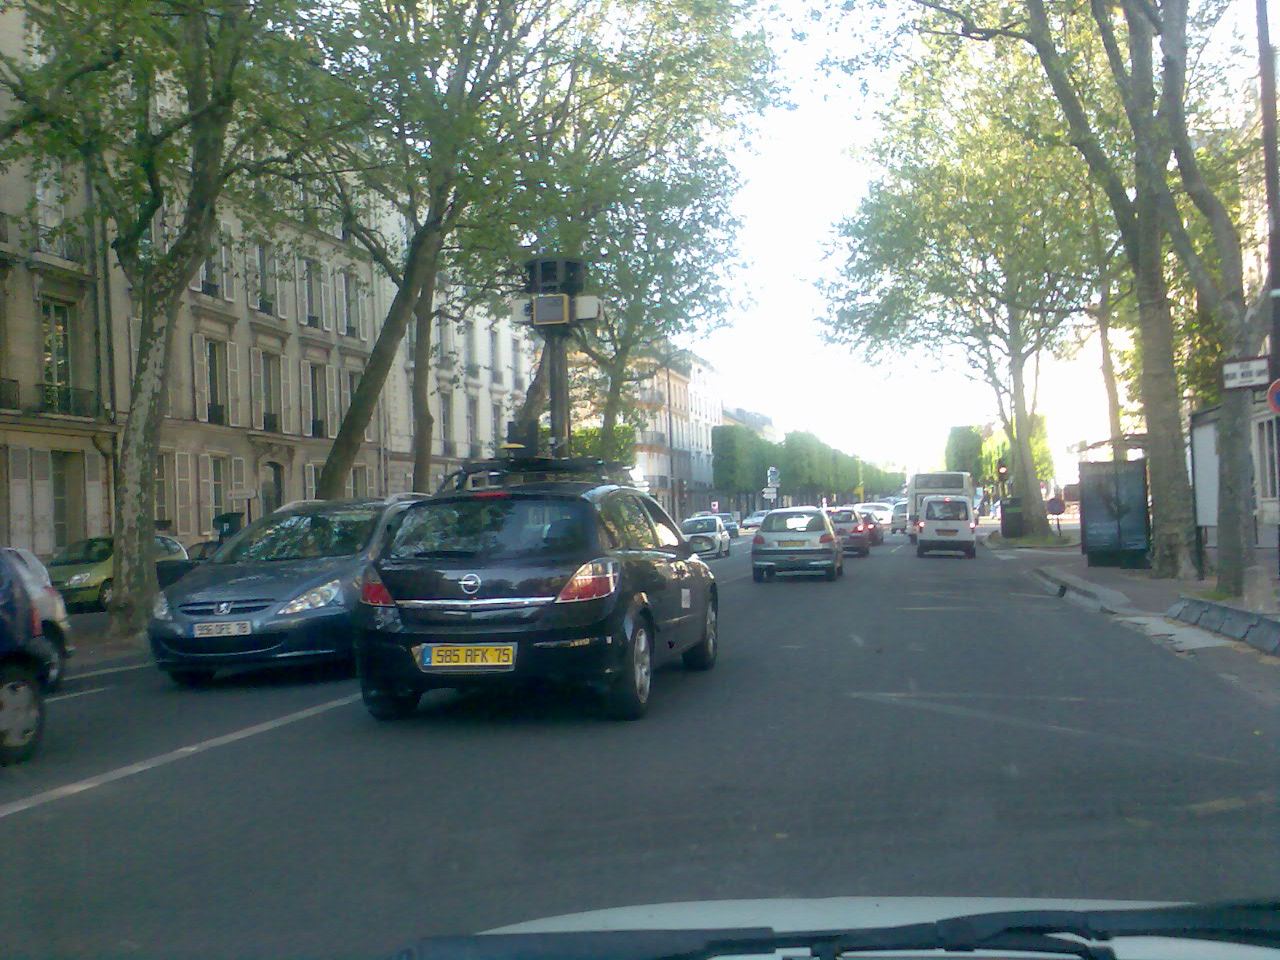
\includegraphics[scale=0.1]{img/fig:street:urban}
		 \end{figure}
		 
		\begin{block}{Problem}
			 Being able to identify the dynamic parts of the environment
		\end{block}
		 
		Constrains
		\begin{itemize}
			\item In a car (platform)
			\item using a laser scanner (sensor)
			\item As fast as possible (online)
		\end{itemize}

		\begin{alertblock}{Not our goal}
			solve DATMO and SLAM
		\end{alertblock}
	\end{frame}


\section{Introduction}

\subsection{Intelligent Transportation Systems}

	\begin{frame}
		\frametitle{Overview}
	
		\begin{figure}[h]
			\center
			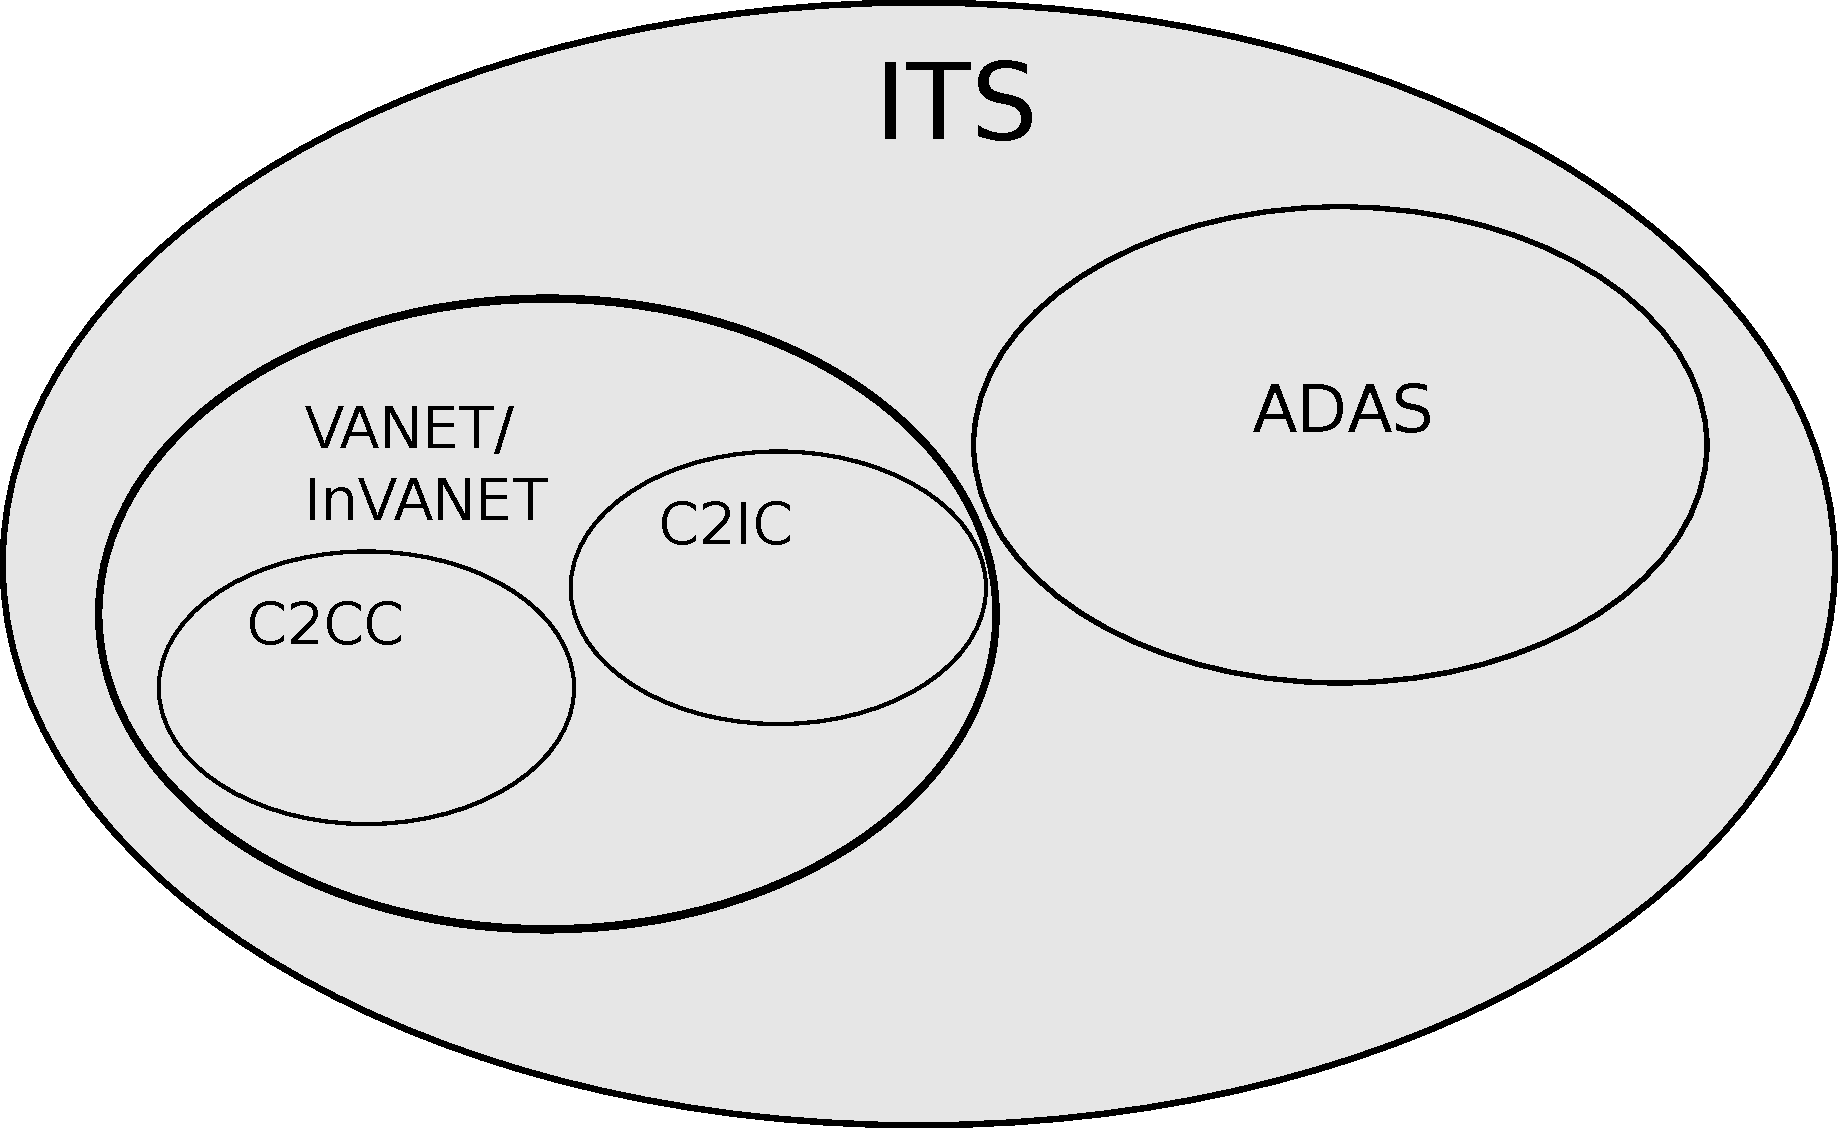
\includegraphics[scale=0.3]{img/fig:its:division}
		 \end{figure}		
		
	\end{frame}

	\begin{frame}
		\frametitle{ADAS}
		
		Advanced Drive Assistance Systems		
		
		\begin{block}{Canonical definition}
			Cope with vehicle handling tasks
		\end{block}		
				
		\begin{block}{Goal}
			\begin{itemize}
			\item Reduce the risk of collisions
			\item Reduce the driver overload
			\item Increase the confort
			\end{itemize}
		\end{block}
		
	\end{frame}

\subsection{Sensors}

	\begin{frame}
		\frametitle{Overview}
	
		\begin{block}{Canonical definition}
			Translate physical \textit{stimuli} in electronic information
		\end{block}
	
		Classified according to?	
		\begin{block}{Definition}
			\begin{itemize}
			\item measurand observed
			\item subject's localization
			\item technology used
			\end{itemize}
		\end{block}			
	
	\end{frame}

	\begin{frame}
		\frametitle{Measurand observed}
		Which kind of physical \textit{stimulus} can be observed?
		\begin{figure}[h]
			\center
			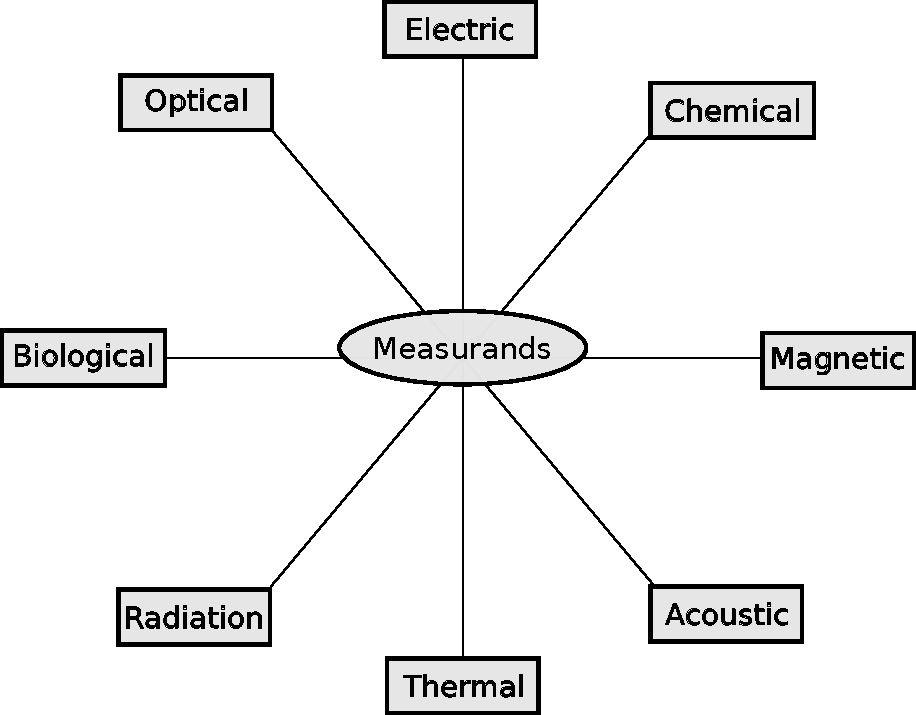
\includegraphics[scale=0.4]{../img/fig:sensors}
		 \end{figure}				
	\end{frame}
	
	\begin{frame}
		\frametitle{subject's localization}
		What we are observing is a property of the moving robot?
		\begin{itemize}
		\item proprioceptive
		\item exteroceptive
		\end{itemize}
		\begin{figure}[h]
			\center
			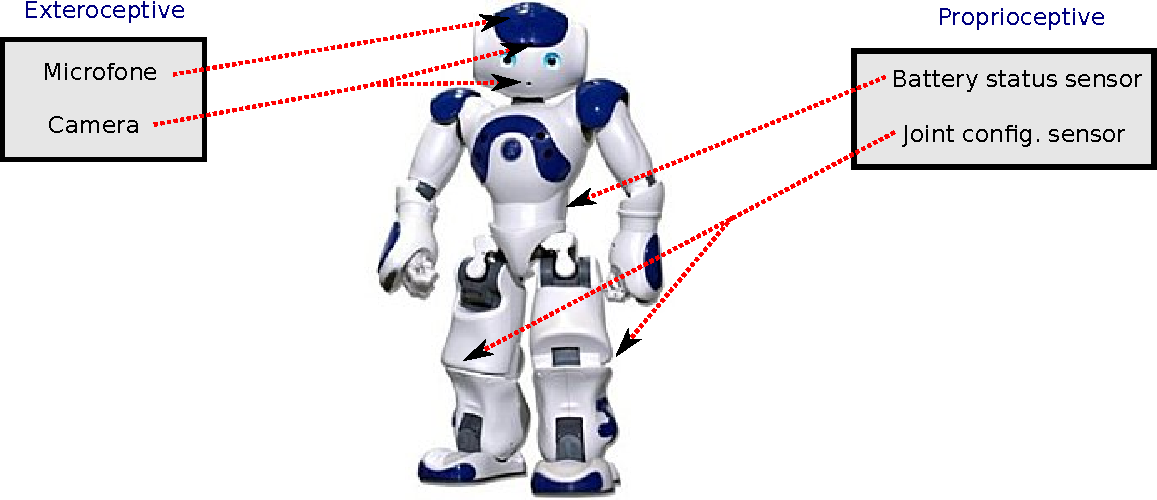
\includegraphics[scale=0.4]{img/fig:nao:config}
		 \end{figure}		
	\end{frame}

	\begin{frame}
		\frametitle{technology used}

		\begin{itemize}
		\item passive
			\begin{itemize}
				\item Emits energy to the enviroment so the measurand can be obtained
				\item e.g. range sensor, radars, etc.
			\end{itemize}		
		\item active
			\begin{itemize}
				\item Receives a physical info and is able to deduce the measurand
				\item e.g. camera, microfone, etc. 
			\end{itemize}		
		
		\end{itemize}		
		
	\end{frame}
	
	\begin{frame}
		\frametitle{What can we say about them?}
			
		\begin{itemize}
			\item Imprecision
			\item Uncertainty
			\item Incomplete data
		\end{itemize}		
		
	\end{frame}

\section{Perception process}

	\begin{frame}
		\frametitle{Overview}
		\begin{block}{Definition}
			The process of acquiring knowledge about the environment \cite{iyengar1991autonomous}
		\end{block}	
		
		\begin{figure}[h]
			\center
			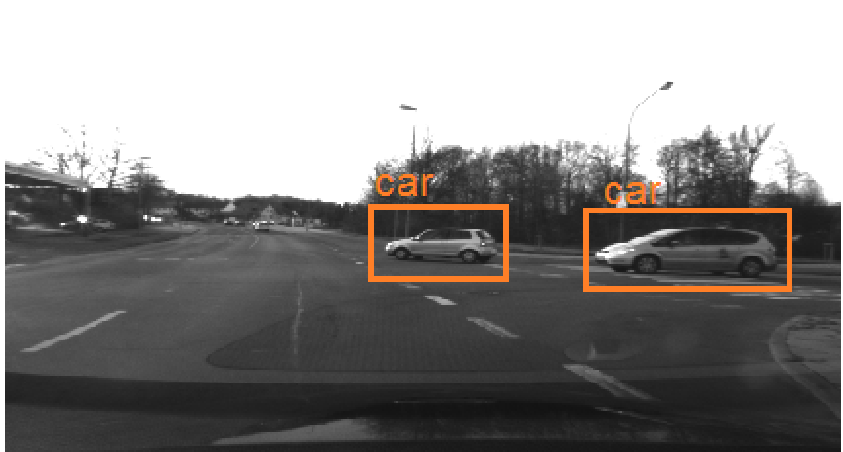
\includegraphics[scale=0.3]{img/fig:perception:ex1}
		 \end{figure}
		 
	\end{frame}

	\begin{frame}
		\frametitle{Grouping process in robotics}
		
		\begin{block}{Goal}		
			Dependable informations are grouped in the same process.
		\end{block}			
		
		\begin{exampleblock}{Process}		
		
			\begin{itemize}
			\item Localization
			\item Mapping
			\end{itemize}			
		
			SLAM
		\end{exampleblock}					
				
		\begin{exampleblock}{Process}		
			\begin{itemize}
			\item Moving objects
				\begin{itemize}
				\item Detection
				\item Tracking
				\end{itemize}			
			\end{itemize}			
			DATMO
		\end{exampleblock}						
				
	\end{frame}

	\subsection{SLAM}
		\begin{frame}
			\frametitle{SLAM}
			
			\begin{block}{Definition}				
				Simultaneous Localization and Mapping
			\end{block}
			
			\begin{figure}[h]
				\center
				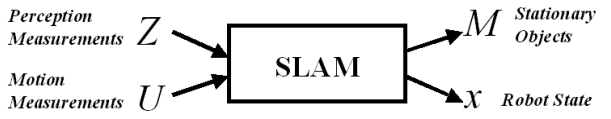
\includegraphics[scale=0.8]{../img/fig:perception:slam}
			 \end{figure}			
			
		\end{frame}
	
	\subsection{DATMO}
		\begin{frame}
			\frametitle{DATMO}
			\begin{block}{Definition}				
				Detection and Tracking of Moving Objects
			\end{block}
			\begin{figure}[h]
				\center
				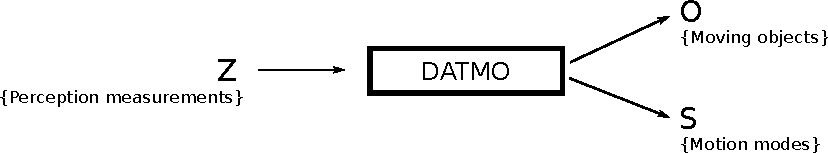
\includegraphics[scale=0.8]{../img/fig:datmo:process}
			 \end{figure}		
		\end{frame}

%%%%%%%%%%%%%%%%%%%%%%%%%%%%%%%%%%%%%

\section{State of the art}

\subsection{Mono-vision}

	\begin{frame}
		\frametitle{Mono-vision}
	\end{frame}

\subsection{Stereo-vision}

	\begin{frame}
		\frametitle{Stereo-vision}
	\end{frame}

\subsection{Laser scanner}

	\begin{frame}
		\frametitle{Laser scanner}
	\end{frame}

\section{Motion Detection}

\subsection{preprocessing}

	\begin{frame}
		\frametitle{Platform}	
		 \begin{columns}[t]
		  \begin{column}{5cm}
		  \begin{figure}[h]
			\center
			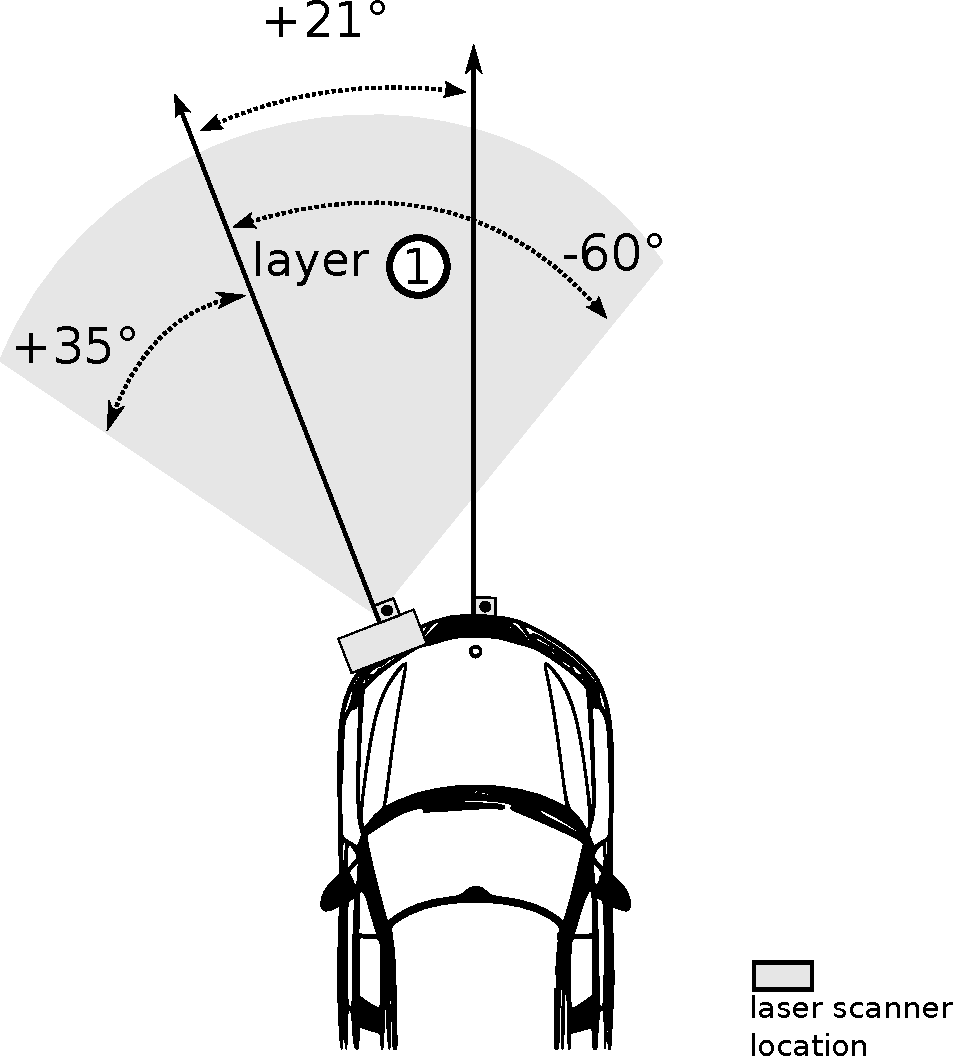
\includegraphics[scale=0.3]{../img/fig:demonstrator:superior}
		  \end{figure}
		  \end{column}
		  
		  \begin{column}{5cm}
		  \begin{figure}[h]
			\center
			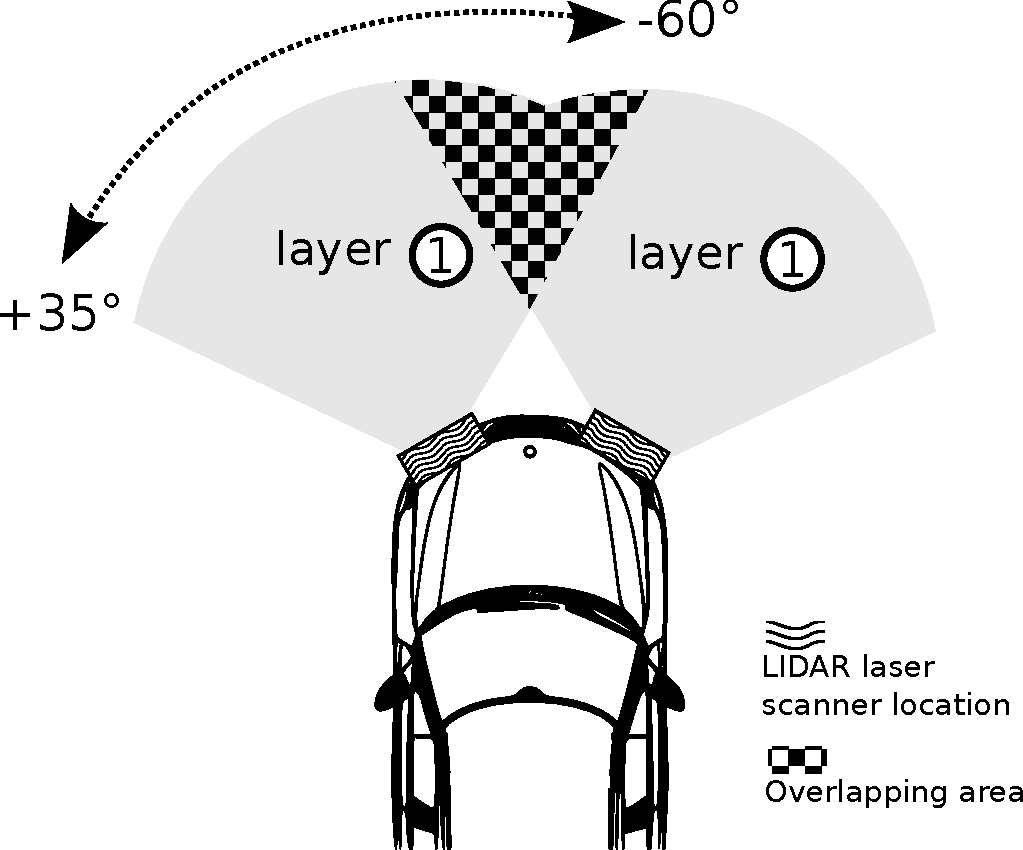
\includegraphics[scale=0.3]{../img/fig:demonstrator:superior:overlap}
		  \end{figure}   
		  \end{column}
		 \end{columns} 	
	
	\end{frame}

	\begin{frame}
		\frametitle{Platform}
		\begin{figure}[h]
			\center
			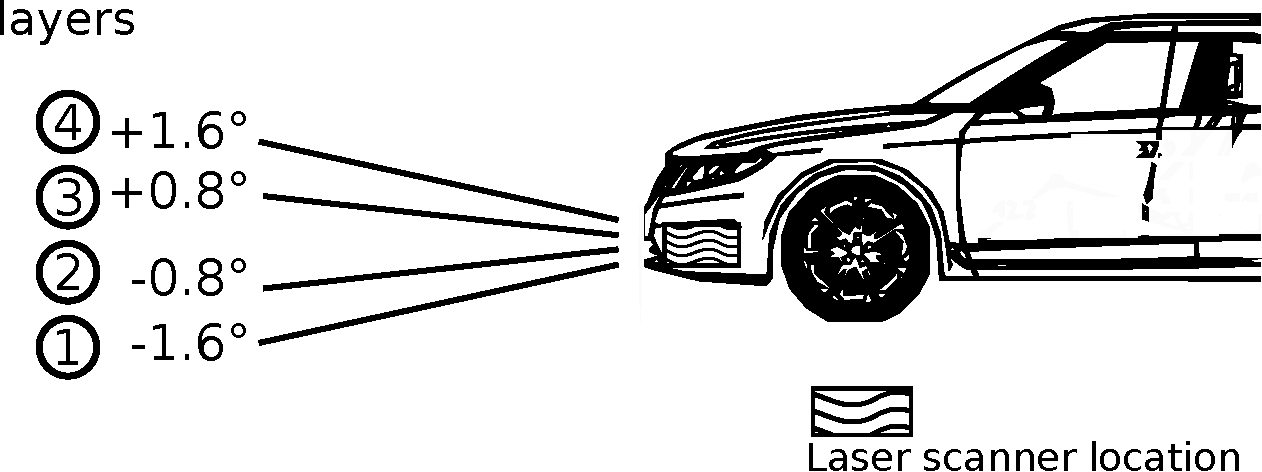
\includegraphics[scale=0.4]{../img/fig:demonstrator:lateral}
		\end{figure}
	\end{frame}

	\begin{frame}
		\frametitle{Input preparation}
		\begin{figure}[h]
			\center
			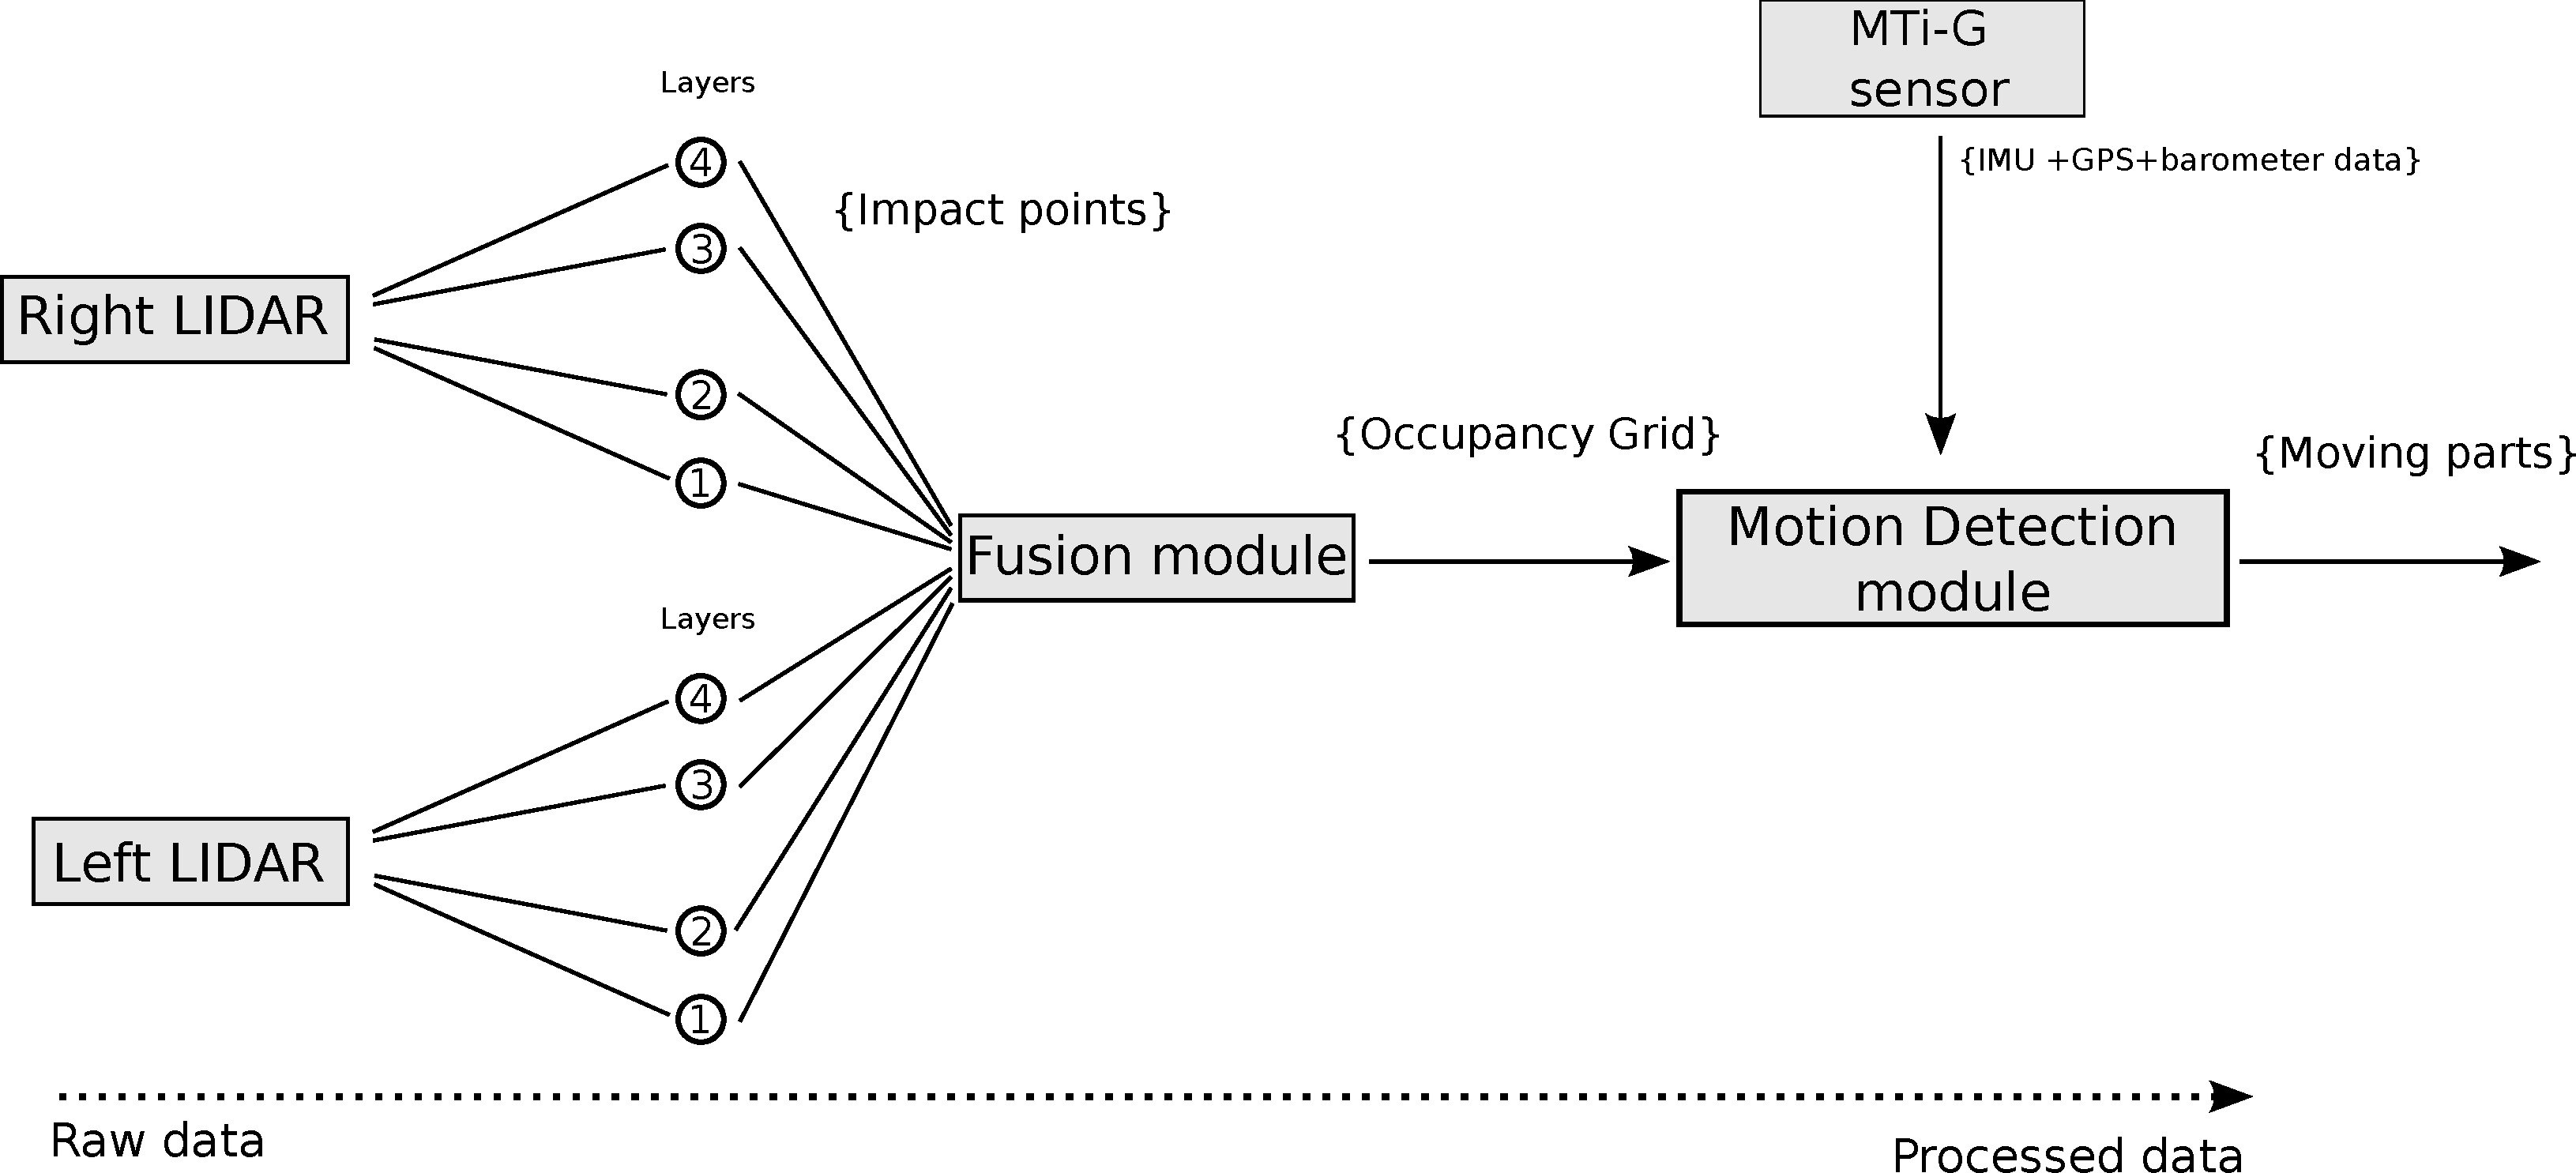
\includegraphics[scale=0.18]{../img/fig:motion:framework}
		\end{figure}
	
	\end{frame}

	\begin{frame}
		\frametitle{Context dependability}
		 
		\begin{block}{In which context}
			Driving assistance systems
		\end{block}
		 
	\end{frame}	

	\begin{frame}
		\frametitle{Solution overview}
		\begin{figure}[h]
			\center
			\includegraphics[scale=0.5]{img/fig:problem}
		 \end{figure}
		 
		\begin{block}{Problem}
			 Being able to identify the dynamic parts of the environment
		\end{block}
		 
		\begin{block}{Result}
			High level classification
		\end{block}				 

		\begin{alertblock}{Not our goal}
			solve DATMO and SLAM
		\end{alertblock}
	\end{frame}

	\begin{frame}
		\frametitle{Pros and Cons}
		
		\begin{block}{Pros}
			\begin{itemize}
			\item easy to integrate with existing solutions
			\item faster way to classify
			\end{itemize}
		\end{block}		
		
		\begin{block}{Cons}
			\begin{itemize}
			\item Need to be filtered afterall to reduce the noise
			\item Directly affect by the quality of the data from the IMU
			\end{itemize}
		\end{block}
		
	\end{frame}

\subsection{algorithm}

\section{Experiments}

\section{Results}

\begin{thebibliography}{9}

	\begin{frame}{References}
		\bibitem{iyengar1991autonomous}
			Iyengar, S.S. and Elfes, A.
			\emph{Autonomous Mobile Robots: Control, planning, and architecture}.
			1991.
			
 	\end{frame}
 	
	\begin{frame}{}
	\begin{alertblock}{}
		\center
		Questions?
	\end{alertblock}
	\end{frame} 	
 	
\end{thebibliography}
 	

\end{document}